\chapter{Observations and Conclusions}
This chapter will discuss the results of the model and the further study that could be done, also the impact of the training data and the limitation of the model.

 \section{Further research}
 This section we will discuss what could be done in the future so that the model will end up with better accuracy to estimate the affine transformation between the aerial images. We will address the research in terms of data and model.
\subsection{Data}
 We developed our own dataset for the purpose of training a machine learning model. However we only ended up using it to test a model that was trained with general images in the same manner as Rocco\cite{Rocco17}. We did try to train our model with this dataset however the model failed to converge. One thing we did not try was to train the model only on subsets of our dataset. Training it with the full set of data, including the rotations and large translations did not allow the model to become useful (the training error was too large). Only during testing and after visually inspecting some examples as we show in Chapter 5 did we develop some subsets of our dataset. It is possible the neural network would train using only our smaller datasets. We leave this for future work.\\
\begin{figure}
\centering
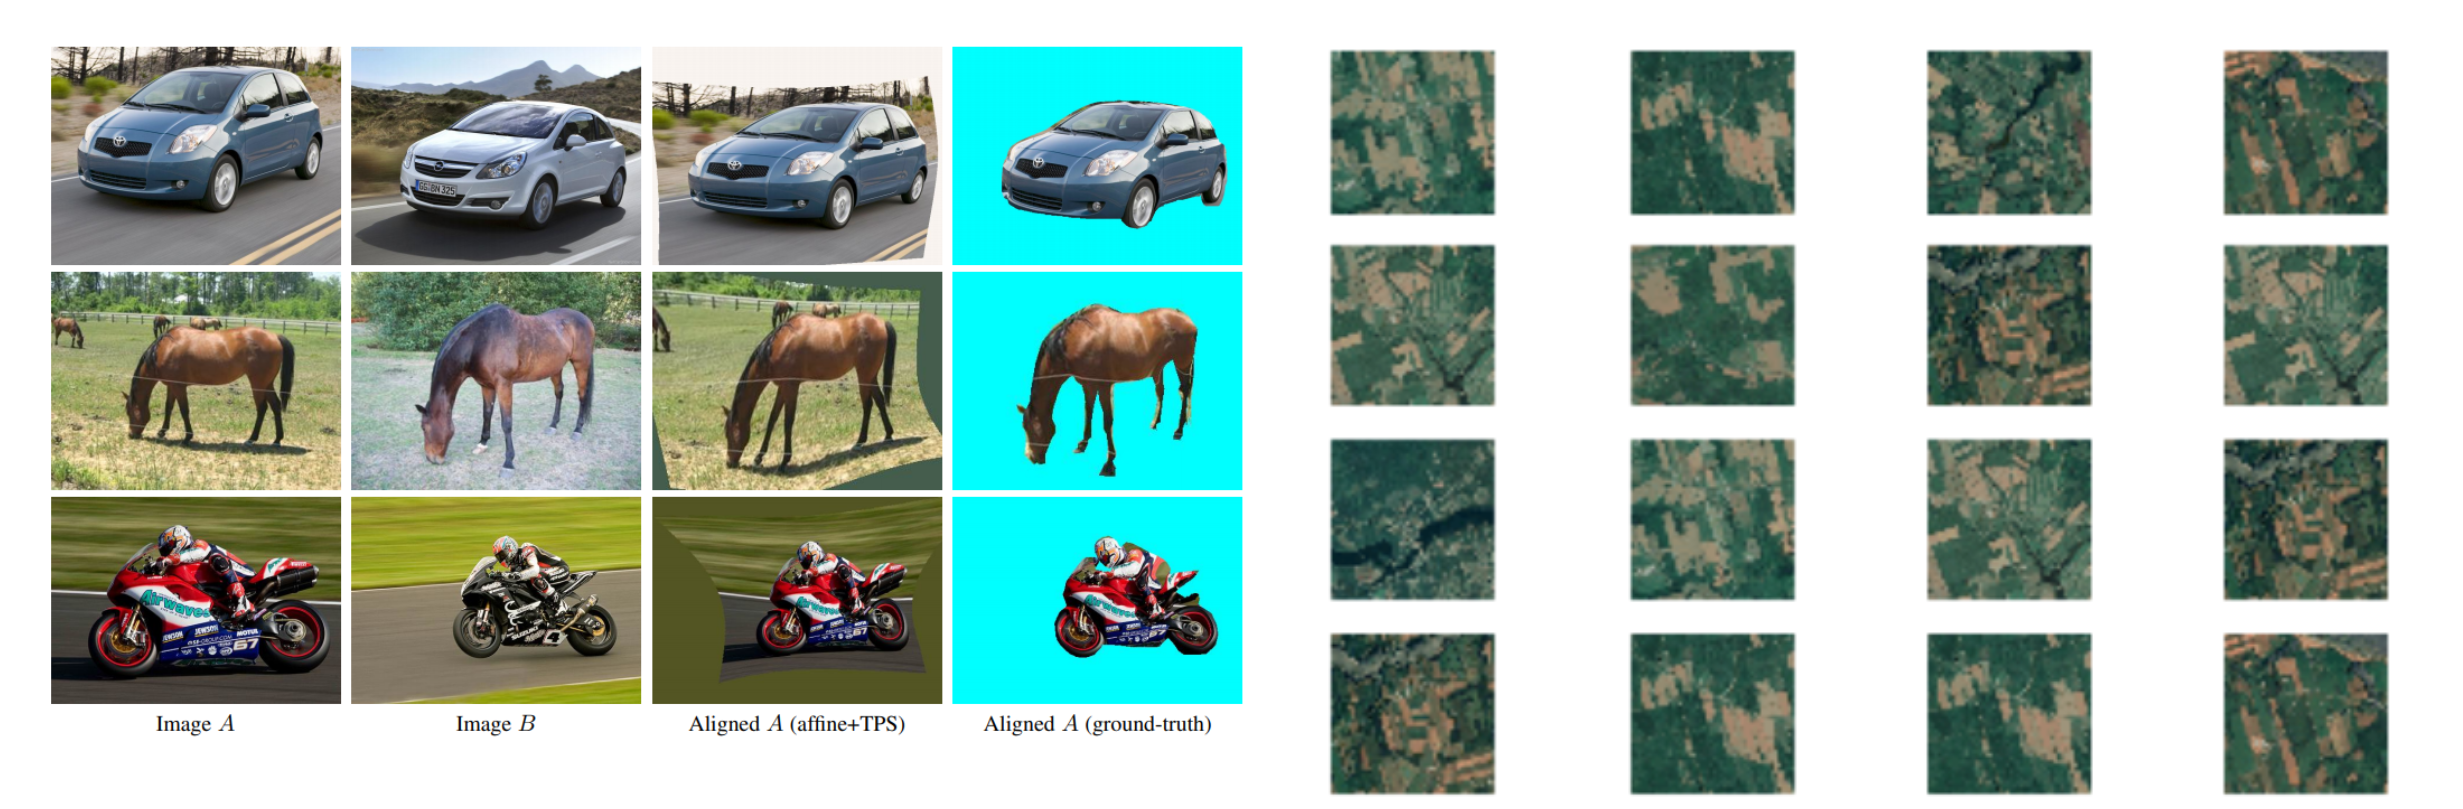
\includegraphics[width = 5.0in]{figs/data_compare}
\caption{The comparison of training data between Rooco,I\citep{Rocco17} and us. The training data from Rocco\citep{Rocco17}(left side) has some key features in the center of the images, but it is not too obvious what is the key features in our training images(right size).}
\end{figure}
 Other thing we could do when we develop the training dataset is try to keep the important feature in both source images and target image so that the model are not struggle finding the features in given image pairs. We developed over 10,000 image pairs to train the models, a datasets contains more than that is likely to help to train the model.
 Figure 6.2 shows one of our image pair that the target image are 60 pixels translate right and 60 pixels translate down.\\

\begin{figure}
\centering
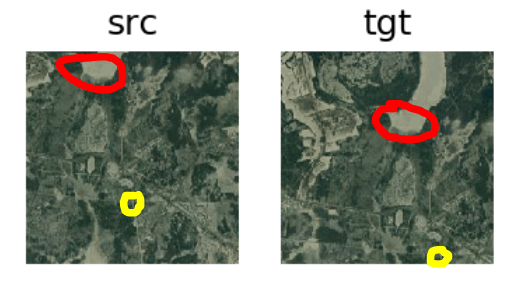
\includegraphics[width = 5.0in]{figs/train_src_tgr}
\caption{This shows a image pair, the target image are 60 pixels translate right and 60 pixels translate down. We circle out the common point in the images, we can see that it is very hard to find strong features between this image pairs even the translation is not too big.}
\end{figure}


\subsection{Model}
 We implement the model from Rocco.I\citep{Rocco17} to estimate only affine transform matrix, the model is working well to do the task, but it is possible to implement other machine learning models that may produce better results. We only implemented the one neural network, while a varied approach may have been beneficial.
\subsubsection{Loss function}
 We are using the MSE(Mean Square Error)\cite{mse} to calculate the error between the truth affine parameters $\theta_{af}$ and the predict affine parameters from the model $\theta_{pred}$.
  The advantage of the MSE is easy to implement and gives us the clear error for our affine transformation and $\theta_{af}$ and the predict affine parameters from the model $\theta_{pred}$. The MSE is a general loss function that works well and suitable for a lot of models for regression problems. \\
  The MSE is not specific for the model. In the model implement by Rocco,I\citep{Rocco17}, they develop the loss function by measuring loss on an imaginary grid of points which is being deformed by the transformation. The following section is form the paper "Convolutional neural network architecture for geometric matching" written by Ricco,I\citep{Rocco17} that gives a clear description of the loss function:
  \begin{quote}
  We construct a grid of points in image A, transform it using the ground truth and neural network estimated transformations $T_{\theta_{GT}}$ and $T_{\theta}$ with parameters $\theta_{GT}$ and $\theta$, respectively, and measure the discrepancy between the two transformed grids by summing the squared distances between the corresponding grid points:
  \begin{align*}
  L(\theta, \theta_{GT})= \frac{1}{N}\sum_{i=1}^{N}{d(T_{\theta}(g_i), T_{\theta_{GT}}(g_i) )}^2
  \end{align*}
  where $g = \{g_i\}=\{(x_i, y_i)\}$ is the uniform grid used, and N = |$g$|. We define the grid as having $x_i,y_i \in \{ s:\ s\ =\ -1\ +\ 0.1\ * n*n  \in \{0,1,2....,20 \} \}$, that is to say, each coordinate belongs to a partition of [-1,1] in equally spaced subintervals of steps 0.1. Note that we construct the coordinate system such that the center of the image is at (0,0) and that the width and height of the image are equal to 2,$i.e$. the bottom left and top right corners have coordinates (-1,-1) and (1,1), respectively.\\
   The gradient of the loss function with respect to the
transformation parameters, needed to perform backpropagation in order to learn network weights, can be computed easily if the location of the transformed grid points $T_{\theta}(g_i)$  is differentiable with respect to $\theta$. This is commonly the case, for example, when T is an affine transformation,
$T_{\theta}(g_i)$ is linear in parameters $\theta$ and therefore the loss can be differentiated in a straightforward manner.
\end{quote}   		
  We have tried to uses this loss function when we training the model with our own dataset, unfortunately just as with MSE, the model did not converge. Thus we were left with a model that did not perform the task. Given the ease of understanding with MSE we kept that cost function for our testing that we presented in Chapter 5

\section{Conclusion}
 We have described a network model that for estimate the affine transformation between the aerial images, the model work well when the source image and the target translation are within 40 pixels, when the image pairs translation go above 40 pixels or involve rotation, the machine learning are struggling produce accurate result.\\ 
   We see the opportunity to modify the training data to produce the better result or implement different model or loss function that the result could comes out more accurate. 